\chapter{Introduction to the \dotNET Framework}
\begin{flushright}
\textit{``The best way to prepare [to be a programmer] is to write programs,}\\
\textit{and to study great programs that other people have written.}\\
\textit{In my case, I went to the garbage cans at the Computer Science Center}\\
\textit{and fished out listings of their operating system.''}
\textit{William Henry Gates III}\\
\end{flushright}

\label{chp:dotnet_platform}

This chapter gives an introduction to the \dotNET Framework of Microsoft. First, the architecture of the \dotNET Framework is introduced. This section includes terms like the Common Language Runtime, the \dotNET Class Library, the Common Language Infrastructure and the Intermediate Language. These are discussed in more detail in the sections following the architecture.

\nomenclature{SOAP}{Simple Object Access Protocol}%
\nomenclature{WSDL}{Web Services Description Language}%
\section{Introduction}
Microsoft defines~\cite{Microsoft03-5} \dotNET as follows; ``\dotNET is the Microsoft Web services strategy to connect information, people, systems, and devices through software.''. There are different \dotNET technologies in various Microsoft products providing the capabilities to create solutions using web services. 
Web services are small, reusable applications that help computers from many different operating system platforms work together by exchanging messages. Based on industry standards like XML (Extensible Markup Language), SOAP (Simple Object Access Protocol), and WSDL (Web Services Description Language) they provide a platform and language independent way to communicate.

Microsoft products, such as Windows Server System (providing web services) or Office System (using web services) are some of the \dotNET technologies. The technology described in this chapter is the \dotNET Framework. Together with Visual Studio, an integrated development environment, they provide the developer tools to create programs for \dotNET. 

Many companies are largely dependent on the \dotNET Framework, but need or want to use AOP. Currently there is no direct support for this in the Framework. The \Compose*[.NET] project is addressing these needs with its implementation of the Composition Filters approach for the \dotNET Framework.

This specific \Compose* version for \dotNET has two main goals.
First, it combines the \dotNET Framework with AOP through Composition Filters.
Second, \Compose* offers superimposition in a language independent manner. The \dotNET Framework supports multiple languages and is, as such, suitable for this purpose.
Composition Filters are an extension of the object-oriented mechanism as offered by \dotNET, hence the implementation is not restricted to any specific object-oriented language.

\section{Architecture of the \dotNET Framework}
\label{sec:OverviewDotNetArchitecture}
\nomenclature{API}{Application Programming Interface}
The \dotNET Framework is Microsoft's platform for building, deploying, and running Web Services and applications. It is designed from scratch and has a consistent API providing support for component-based programs and Internet programming.
This new Application Programming Interface (API) has become an integral component of Windows. The \dotNET Framework was designed to fulfill the following objectives~\cite{Microsoft03-1}:

\begin{description}[noitemsep, style=nextline]
  \item[Consistency] Allow object code to be stored and executed locally, executed locally but Internet-distributed, or executed remotely and to make the developer experience consistent across a wide variety of types of applications, such as Windows-based applications and Web-based applications;
  \item[Operability] The ease of operation is enhanced by minimizing version conflicts and providing better software deployment support;
  \item[Security] All the code is executed safely, including code created by an unknown or semi-trusted third party;
  \item[Efficiency] The \dotNET Framework compiles applications to machine code before running thus eliminating the performance problems of scripted or interpreted environments;
  \item[Interoperability] Code based on the \dotNET Framework can integrate with other code because all communication is built on industry standards.
\end{description}

\begin{figure}
 \centering
 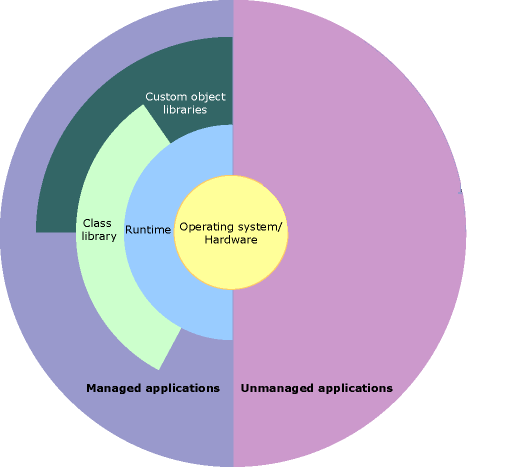
\includegraphics[style=thirdheight]{dotNET_context}
 \caption[Context of the \dotNET framework]{Context of the \dotNET Framework (Modified)~\cite{Microsoft03-1}}
 \label{fig:dotNET_context}
\end{figure}

\nomenclature{CLR}{Common Language Runtime}%
\nomenclature{CTS}{Common Type System}%
\nomenclature{CLS}{Common Language Specification}%
\nomenclature{FCL}{Framework Class Library}%
\nomenclature{CLI}{Common Language Infrastructure}%
The \dotNET Framework consists of two main components~\cite{Microsoft03-1}: the Common Language Runtime (CLR, simply called the \dotNET Runtime or Runtime for short) and the \dotNET Framework Class Library (FCL). 
The CLR is the foundation of the \dotNET Framework, executing the code and providing the core services such as memory management, thread management and exception handling. The CLR is described in more detail in \autoref{sec:clr}.
The class library, the other main component of the \dotNET Framework, is a comprehensive, object-oriented collection of reusable types that can be used to develop applications ranging from traditional command-line or graphical user interface (GUI) applications to applications such as Web Forms and XML Web services. \autoref{sec:fcl} describes the class libraries in more detail.

The code run by the runtime is in a format called Common Intermediate Language (CIL), further explained in~\autoref{sec:TheIntermediateLanguage}. The Common Language Infrastructure (CLI) is an open specification that describes the executable code and runtime environment that form the core of the Microsoft \dotNET Framework. \autoref{sec:cts} tells more about this specification.

\autoref{fig:dotNET_context} shows the relationship of the \dotNET Framework to other applications and to the complete system. The two parts, the class library and the runtime, are managed, \ie applications managed during execution. The operating system is in the core, managed and unmanaged applications operate on the hardware. The runtime can us other object libraries and the class library, but the other libraries can use the same class library them self.

Besides the Framework, Microsoft also provides a developer tool called the Visual Studio. This is an IDE with functionality across a wide range of areas allowing developers to build applications with decreased development time in comparison with developing applications using command line compilers.

\subsection{Version 2.0 of \dotNET}
\label{sec:Version2}
In November 2005, Microsoft released a successor of the \dotNET Framework. 
Major changes are the support for generics, the addition of nullable types, 64 bit support, improvements in the garbage collector, new security features and more network functionality.

Generics make it possible to declare and define classes, structures, interfaces, methods and delegates with unspecified or generic type parameters instead of specific types.
When the generic is used, the actual type is specified.
This allows for type-safety at compile-time.
Without generics, the use of casting or boxing and unboxing decreases performance.
By using a generic type, the risks and costs of these operations is reduced.

Nullable types allow a value type to have a normal value or a null value.
This null value can be useful for indicating that a variable has no defined value because the information is not currently available.

Besides changes in the Framework, there are also improvements in the four main Microsoft \dotNET programming languages (C\#, VB\dotNET, J\# and C++).
The language elements are now almost equal for all languages.
For instance, additions to the Visual Basic language are the support for unsigned values and new operators and additions to the C\# language include the ability to define anonymous methods thus eliminating the need to create a separate method.

A new Visual Studio 2005 edition was released to support the new Framework and functionalities to create various types of applications.

\section{Common Language Runtime}
\label{sec:clr}
The Common Language Runtime executes code and provides core services. These core services are memory management, thread execution, code safety verification and compilation. Apart from providing services, the CLR also enforces code access security and code robustness. 
Code access security is enforced by providing varying degrees of trust to components, based on a number of factors, \eg the origin of a component. 
This way, a managed component might or might not be able to perform sensitive functions, like file-access or registry-access. 
By implementing a strict type-and-code-verification infrastructure, called the Common Type System (CTS), the CLR enforces code robustness. Basically there are two types of code; 

\begin{description}[noitemsep,style=nextline]
\item[Managed]
Managed code is code, which has its memory handled and its types validated at execution by the CLR.
It has to conform to the Common Type Specification (CTS \autoref{sec:cts}).
If interoperability with components written in other languages is required, managed code has to conform to an even more strict set of specifications, the Common Language Specification (CLS).
The code is run by the CLR and is typically stored in an intermediate language format. This platform independent intermediate language is officially known as Common Intermediate Language (CIL \autoref{sec:TheIntermediateLanguage})~\cite{Watkins00}.
\item[Unmanaged]
Unmanaged code is not managed by the CLR. It is stored in the native machine language and is not run by the runtime but directly by the processor.
\end{description}
\nomenclature{JIT}{Just-in-time}

All language compilers (targeting the CLR) generate managed code (CIL) that conforms to the CTS. 

At runtime, the CLR is responsible for generating platform specific code, which can actually be executed on the target platform.
Compiling from CIL to the native machine language of the platform is executed by the just-in-time (JIT) compiler. Because of this language independent layer it allows the development of CLRs for any platform, creating a true interoperability infrastructure~\cite{Watkins00}.
The \dotNET Runtime from Microsoft is actually a specific CLR implementation for the Windows platform.
\nomenclature{PDA}{Personal Digital Assistant}
Microsoft has released the \emph{\dotNET Compact Framework} especially for devices such as personal digital assistants (PDAs) and mobile phones.
The \dotNET Compact Framework contains a subset of the normal \dotNET Framework and allows \dotNET developer to write mobile applications. Components can be exchanged and web services can be used so an easier interoperability between mobile devices and workstations/servers can be implemented~\cite{Microsoft03-3}.

At the time of writing, the \dotNET Framework is the only advanced Common Language Infrastructure (CLI) implementation available.
A shared-source\footnote{Only non-commercial purposes are allowed.} implementation of the CLI for research and teaching purposes was made available by Microsoft in 2002 under the name Rotor~\cite{Stutz02}. In 2006 Microsoft released an updated version of Rotor for the \dotNET platform version two.
Also Ximian is working on an open source implementation of the CLI under the name Mono\footnote{\url{http://www.go-mono.com/}}, targeting both Unix/Linux and Windows platforms.
Another, somewhat different approach, is called Plataforma.NET\footnote{\url{http://personals.ac.upc.edu/enric/PFC/Plataforma.NET/p.net.html}} and aims to be a hardware implementation of the CLR, so that CIL code can be run natively.

\subsection{Java VM vs \dotNET CLR}
There are many similarities between Java and \dotNET technology. This is not strange, because both products serve the same market.

\nomenclature{JVM}{Java Virtual Machine}
Both Java and \dotNET are based on a runtime environment and an extensive development framework.
These development frameworks provide largely the same functionality for both Java and \dotNET.
The most obvious difference between them is lack of language independence in Java.
While Java's strategy is `One language for all platforms' the \dotNET philosophy is `All languages on one platform'.
However these philosophies are not as strict as they seem.
As noted in \autoref{sec:fcl} there is no technical obstacle for other platforms to implement the \dotNET Framework.
There are compilers for non-Java languages like Jython (Python)~\cite{Jython03} and WebADA~\cite{Ada96} available for the JVM.
Thus, the JVM in its current state, has difficulties supporting such a vast array of languages as the CLR.
However, the multiple language support in \dotNET is not optimal and has been the target of some criticism.

Although the JVM and the CLR provide the same basic features they differ in some ways.
While both CLR and the modern JVM use JIT (Just In Time) compilation the CLR can directly access native functions.
This means that with the JVM an indirect mapping is needed to interface directly with the operating system.
\section{Common Language Infrastructure}
\label{sec:cts}
The entire CLI has been documented, standardized and approved~\cite{Ecma-335} by the European association for standardizing information and communication systems, Ecma International\footnote{An European industry association founded in 1961 and dedicated to the standardization of Information and Communication Technology (ICT) Systems.
Their website can be found at \url{http://www.ecma-international.org/}.}.
Benefits of this CLI for developers and end-users are:

\begin{itemize}[noitemsep]
  \item Most high level programming languages can easily be mapped onto the Common Type System (CTS);
  \item The same application will run on different CLI implementations;
  \item Cross-programming language integration, if the code strictly conforms to the Common Language Specification (CLS);
  \item Different CLI implementations can communicate with each other, providing applications with easy cross-platform communication means.
\end{itemize}

This interoperability and portability is, for instance, achieved by using a standardized meta data and intermediate language (CIL) scheme as the storage and distribution format for applications.
In other words, (almost) any programming language can be mapped to CIL, which in turn can be mapped to any native machine language.

The Common Language Specification is a subset of the Common Type System, and defines the basic set of language features that all \dotNET languages should adhere to.
In this way, the CLS helps to enhance and ensure language interoperability by defining a set of features that are available in a wide variety of languages.
The CLS was designed to include all the language constructs that are commonly needed by developers 
(\eg naming conventions, common primitive types), but no more than most languages are able to support~\cite{Microsoft03-2}.
\autoref{fig:Common_Type_System} shows the relationships between the CTS, the CLS, and the types available in C++ and C\#.
\begin{figure}
 \centering
 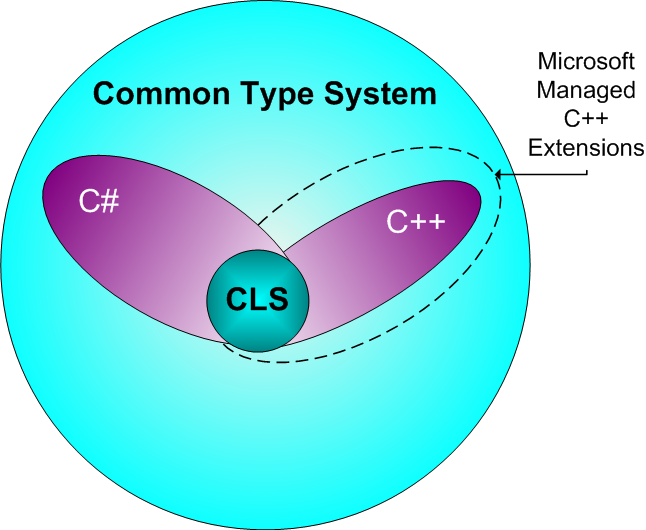
\includegraphics[style=fourthheight]{Common_Type_System}
 \caption{Relationships in the CTS}
 \label{fig:Common_Type_System}
\end{figure}
In this way the standardized CLI provides, in theory\footnote{Unfortunately Microsoft did not submit all the framework classes for approval and at the time of writing only the \dotNET Framework implementation is stable.}, a true cross-language and cross-platform development and runtime environment.

To attract a large number of developers for the \dotNET Framework, Microsoft has released CIL compilers for C++, C\#, J\#, and VB.NET.
In addition, third-party vendors and open-source projects also released compilers targeting the \dotNET Framework, such as Delphi.NET, Perl.NET, IronPython, and Eiffel.NET.
These programming languages cover a wide-range of different programming paradigms, such as classic imperative, object-oriented, scripting, and declarative languages. This wide coverage demonstrates the power of the standardized CLI.

\begin{figure}
 \centering
 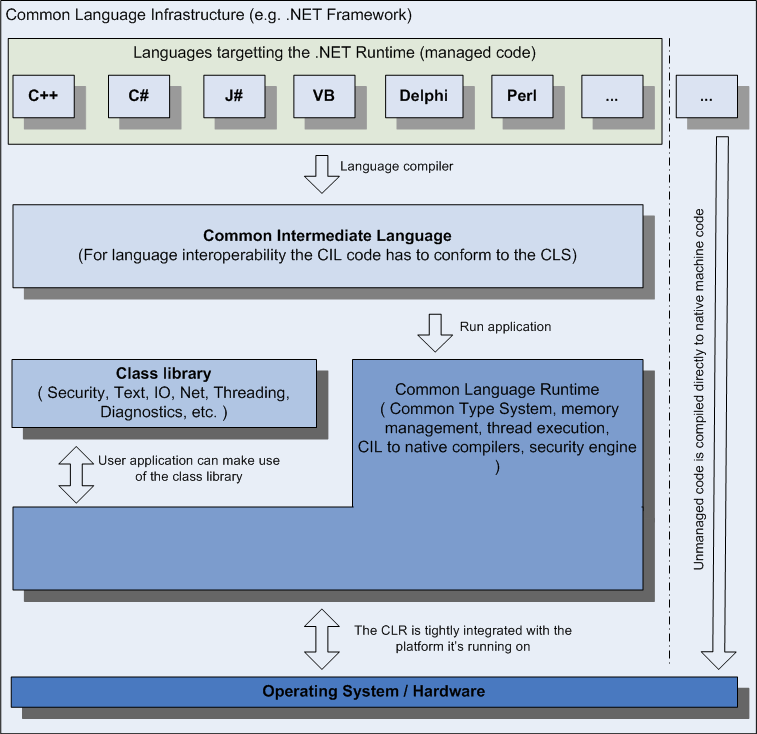
\includegraphics[style=halfheight]{Common_Language_Infrastructure}
 \caption[Main components of the CLI and their relationships]{%
    Main components of the CLI and their relationships.
    The right hand side of the figure shows the difference between managed code and unmanaged code.}
 \label{fig:Common_Language_Infrastructure}
\end{figure}

\autoref{fig:Common_Language_Infrastructure} shows the relationships between all the main components of the CLI.
The top of the figure shows the different programming languages with compiler support for the CLI. Because the compiled code is stored and distributed in the Common Intermediate Language format, the code can run on any CLR. For cross-language usage this code has to comply with the CLS.
Any application can use the class library (the FCL) for common and specialized programming tasks. 
\section{Framework Class Library}
\label{sec:fcl}
The \dotNET Framework class library is a comprehensive collection of object-oriented reusable types for the CLR. 
This library is the foundation on which all the \dotNET applications are built.
It is object oriented and provides integration of third-party components with the classes in the \dotNET Framework.
Developers can use components provided by the \dotNET Framework, other developers and their own components.
\nomenclature{GUI}{Graphical User Interface}%
\nomenclature{XML}{eXtensible Markup Language}%
A wide range of common programming tasks (\eg string management, data collection, reflection, graphics, database connectivity or file access) can be accomplished easily by using the class library.
Also, a great number of specialized development tasks are extensively supported, like:
\begin{itemize}[noitemsep]
  \item Console applications;
  \item Windows GUI applications (Windows Forms);
  \item Web applications (Web Forms);
  \item XML Web services;
  \item Windows services.
\end{itemize}
All the types in this framework are CLS compliant and can therefore be used from any programming language whose compiler conforms to the Common Language Specification (CLS).
\section{Common Intermediate Language}
\label{sec:TheIntermediateLanguage}
The Common Intermediate Language (CIL) has already been mentioned briefly in the sections before, but this section will describe the IL in more detail.
All the languages targeting the \dotNET Framework compile to this CIL (see \autoref{fig:Overview_of_the_Common_Language_Infrastructure}).

\begin{figure}[htbp]
  \centering
  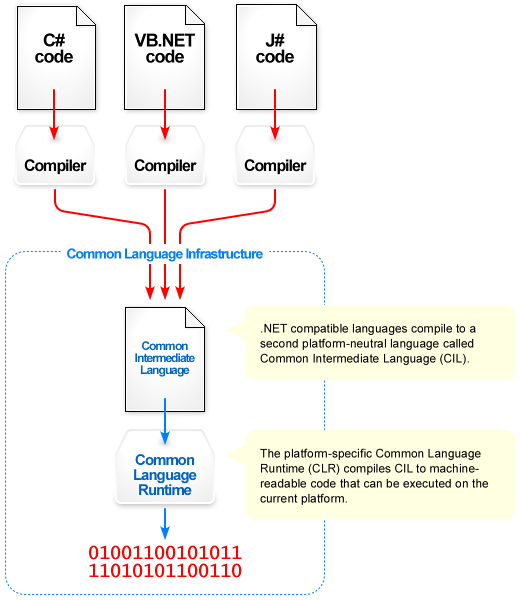
\includegraphics[style=halfheight]{Overview_of_the_Common_Language_Infrastructure}
  \caption{From source code to machine code}
  \label{fig:Overview_of_the_Common_Language_Infrastructure}
\end{figure}

A \dotNET compiler generates a \emph{managed module} which is an executable designed to be run by the CLR~\cite{Prosise2002}.
There are four main elements inside a managed module:

\begin{itemize}[noitemsep]
  \item A Windows Portable Executable (PE) file header;
  \item A CLR header containing important information about the module, such as the location of its CIL and metadata;
  \item Metadata describing everything inside the module and its external dependencies;
  \item The CIL instructions generated from the source code.
\end{itemize}

The Portable Executable file header allows the user to start the executable.
This small piece of code will initiate the just-in-time compiler which compiles the CIL instructions to native code when needed, while using the metadata for extra information about the program.
This native code is machine dependent while the original IL code is still machine independent.
This way the same IL code can be JIT-compiled and executed on any supported architecture.
The CLR cannot use the managed module directly but needs an assembly. 

An assembly is the fundamental unit of security, versioning, and deployment in the \dotNET Framework and is a collection of one or more files grouped together to form a logical unit~\cite{Prosise2002}.
Besides managed modules inside an assembly, it is also possible to include resources like images or text.
A manifest file is contained in the assembly describing not only the name, culture and version of the assembly but also the references to other files in the assembly and security requests.

\nomenclature{OpCode}{Operation Code}%
The CIL is an object oriented assembly language with around 100 different instructions called OpCodes.
It is stack-based, meaning objects are placed on an evaluation stack before the execution of an operation, and when applicable, the result can be found on the  stack after the operation.
For instance, when adding two numbers, first those numbers have to be placed onto the stack, second the add operation is called and finally the result can be retrieved from the stack.

\begin{lstlisting}[language=CIL,style=listing,caption={Adding example in IL code},label={lst:ilexample}]
.assembly AddExample {}

.method static public void main() il managed
{
  .entrypoint           // entry point of the application
  .maxstack 2

  ldc.i4 3              // Place a 32-bit (i4) 3 onto the stack
  ldc.i4 7              // Place a 32-bit (i4) 7 onto the stack
	
  add                   // Add the two and 
	                      // leave the sum on the stack
  
  // Call static System.Console.Writeline function
  // (function pops integer from the stack)
  call void [mscorlib]System.Console::WriteLine(int32)

  ret
}
\end{lstlisting}

To illustrate how to create a \dotNET program in IL code we use the previous example of adding two numbers and show the result.
In \autoref{lst:ilexample} a new assembly is created with the name \lstinline|AddExample|.
In this assembly a function \lstinline|main| is declared as the starting point (\lstinline|entrypoint|) of this assembly.
The \lstinline|maxstack| command indicates there can be a maximum of two objects on the stack and this is enough for the example method.
Next, the values 3 and 7 are placed onto the stack. The \lstinline|add| operation is called and the results stays on the stack.
The method \lstinline|WriteLine| from the \dotNET Framework Class Library is called.
This method resides inside the \lstinline|Console| class placed in the \lstinline|System| assembly.
It expects one parameter with a \lstinline|int32| as its type that will be retrieved from the stack.
The \lstinline|call| operation will transfer the control flow to this method passing along the parameters as objects on the stack.
The \lstinline|WriteLine| method does not return a value.
The \lstinline|ret| operation returns the control flow from the main method to the calling method, in this case the runtime.
This will exit the program.

To be able to run this example, we need to compile the IL code to bytecode where each OpCode is represented as one byte.
To compile this example, save it as a text file and run the \emph{ILASM} compiler with as parameter the filename.
This will produce an executable runnable on all the platforms where the \dotNET Framework is installed.

This example was written directly in IL code, but we could have used a higher level language such as C\# or VB\dotNET. For instance, the same example in C\# code is shown in~\autoref{lst:CSharpAddExample} and the VB\dotNET version is listed in~\autoref{lst:VBAddExample}. When this code is compiled to IL, it will look like the code in~\autoref{lst:ilexample}.

\begin{lstlisting}[language={[Sharp]C},style=listing,caption={Adding example in the C\# language},label={lst:CSharpAddExample}]
public static void main()
{
      Console.WriteLine((int) (3 + 7));
} 
\end{lstlisting} 

\begin{lstlisting}[language={[Visual]{Basic}},style=listing,caption={Adding example in the VB\dotNET language},label={lst:VBAddExample}]
Public Shared Sub main()
      Console.WriteLine(CType((3 + 7), Integer))
End Sub
\end{lstlisting} 

 

